\documentclass{article}

\usepackage{fullpage}
\usepackage{amsmath}
\usepackage{graphicx}
\usepackage{hyperref}
\usepackage{xepersian}

\newcommand{\assignment}{مینی پروژه اول}
\newcommand{\course}{مبانی سیستم‌های هوشمند\\}
\newcommand{\faculty}{دانشکده مهندسی برق\\}
\newcommand{\university}{دانشگاه صنعتی خواجه نصیرالدین طوسی\\}

\hypersetup{colorlinks=true, linkcolor=blue, urlcolor=magenta}

\settextfont[Path={fonts/}, BoldFont={IRLotusICEE_Bold.ttf}, BoldItalicFont={IRLotusICEE_BoldIranic.ttf}, ItalicFont={IRLotusICEE_Iranic.ttf}, Scale=1.2]{IRLotusICEE.ttf}
\setlatintextfont[Path=fonts/, BoldFont={LiberationSerif-Bold.ttf}, BoldItalicFont={LiberationSerif-BoldItalic.ttf}, ItalicFont={LiberationSerif-Italic.ttf}, Scale=1]{LiberationSerif-Regular.ttf}

\title{\assignment}
\author{
    محمدمهدی کرمی \\
    \texttt{mmehdi.karami@email.kntu.ac.ir}
}
\date{\university
\faculty
\course}

\begin{document}

\maketitle

\section{پرسش اول}

لینک گیت‌هاب: \href{https://github.com/username/repository}{سیستم‌های هوشمند}

\subsection{پرسش اول - بخش اول}
این مجموعه داده مربوط به مشتریان یک بانک است که هدف آن پیش‌بینی ترک مشتریان از خدمات کارت اعتباری است. در این مجموعه، داده‌ها شامل سن، وضعیت تأهل، محدودیت اعتبار کارت، و دسته‌بندی کارت اعتباری جمع‌آوری شده‌اند. هدف اصلی از استفاده از این مجموعه داده، پیش‌بینی احتمال ترک مشتریان (churn) است تا بانک بتواند به صورت پیشگیرانه اقدامات لازم را انجام دهد و مشتریان خود را حفظ کند.

در ابتدا، طبق توضیحات داده شده، باید دو ستون آخر که مربوط به پیش‌بینی هستند را نادیده بگیریم، زیرا این مدل به این ستون‌ها نیاز ندارد و برای تجزیه و تحلیل باید حذف شوند.

ویژگی‌های این مجموعه داده عبارتند از:
شناسه مشتری، پرچم ترک مشتری، سن مشتری، جنسیت، تعداد افراد تحت تکفل، سطح تحصیلات، وضعیت تأهل، دسته‌بندی درآمد، دسته‌بندی کارت اعتباری، تعداد ماه‌ها با بانک، تعداد ارتباطات با بانک، تعداد ماه‌های غیرفعال در ۱۲ ماه گذشته، تعداد تماس‌ها با بانک در ۱۲ ماه گذشته، محدودیت اعتبار کارت اعتباری، مجموع موجودی‌های کارت، تغییرات در مجموع مبلغ تراکنش‌ها، تعداد تراکنش‌ها، و تغییرات در تعداد تراکنش‌ها.

تعداد نمونه‌ها در این مجموعه داده ۱۰,۱۲۷ است.

\subsection{پرسش اول - بخش دوم}
پنج ویژگی سن، محدودیت اعتبار کارت اعتباری، مجموع موجودی‌های کارت، مجموع مبلغ تراکنش‌های انجام‌شده، و میانگین نسبت استفاده از اعتبار را انتخاب کرده و بخش داده را نمایش خواهیم داد.

\begin{figure}[!h]
    \centering
    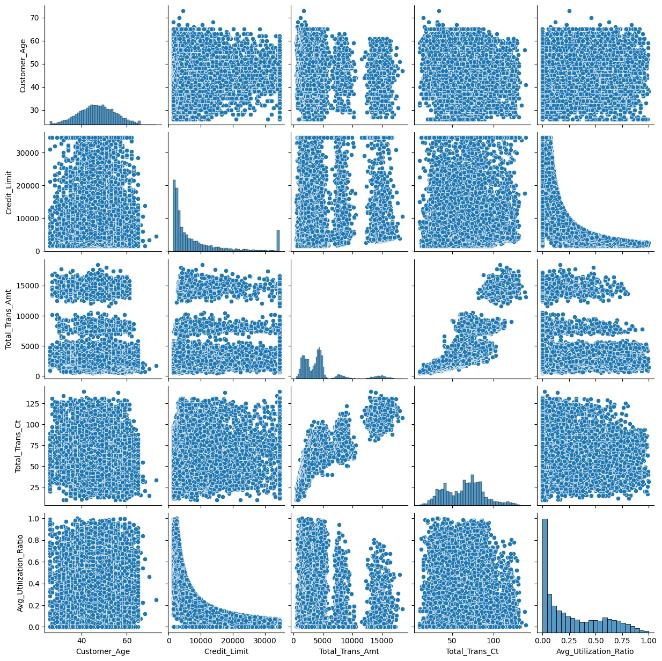
\includegraphics[width=0.4\textwidth]{img/1.png}
\end{figure}

\subsection{پرسش اول - بخش سوم}
جنسیت، وضعیت تأهل، مجموع موجودی‌های کارت و محدودیت اعتبار کارت اعتباری را انتخاب کرده و همبستگی میان آنها را به صورت نموداری نمایش خواهیم داد.

\begin{figure}[!h]
    \centering
    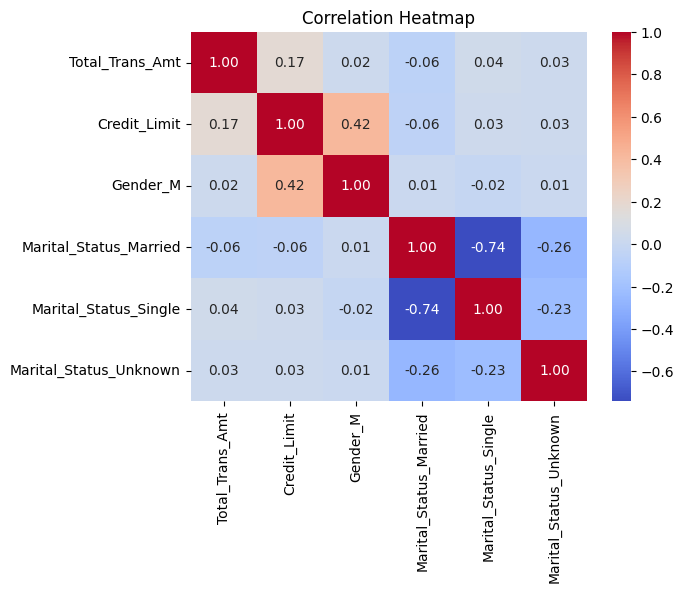
\includegraphics[width=0.4\textwidth]{img/2.png}
\end{figure}

\subsection{پرسش اول - بخش چهارم}
قبل از حذف مقادیر مفقود (NaN)، مجموعه داده شامل ۱۰,۱۲۷ ردیف و ۲۱ ستون بود. پس از حذف ردیف‌هایی که دارای مقادیر NaN بودند، تعداد ردیف‌ها به ۷,۰۸۱ کاهش یافت و تعداد ستون‌ها همچنان ثابت ماند. این تغییر نشان‌دهنده حذف ۳,۰۴۶ ردیف از داده‌ها به دلیل وجود مقادیر مفقود است. مقادیر مفقود در سه ستون \texttt{level\_education} (۱۵۱۹ مقدار مفقود)، \texttt{status\_marital} (۷۴۹ مقدار مفقود) و \texttt{category\_income} (۱۱۱۲ مقدار مفقود) وجود داشتند.

\subsection{پرسش اول - بخش پنجم}
ویژگی \texttt{Attrition\_Flag} دو کلاس دارد: مشتری موجود (۸,۵۰۰ نمونه) و مشتری ترک کرده (۱,۶۲۷ نمونه). توزیع داده موجود در این ویژگی را به صورت یک نمودار دایره‌ای نمایش خواهیم داد.

\begin{figure}[!h]
    \centering
    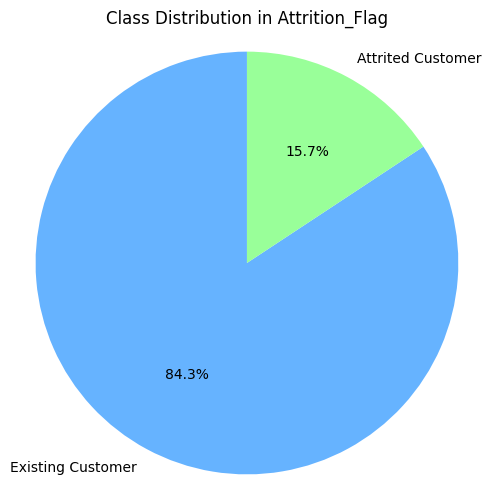
\includegraphics[width=0.4\textwidth]{img/3.png}
\end{figure}

عدم تعادل در داده‌ها، مانند ویژگی \texttt{Flag\_Attrition}، می‌تواند باعث بروز مشکلاتی در عملکرد مدل‌های یادگیری ماشین شود، زیرا مدل تمایل دارد پیش‌بینی‌های خود را به سمت کلاس اکثریت متمایل کند. این امر باعث می‌شود که مدل نتواند به خوبی کلاس اقلیت را شناسایی کند و دقت پیش‌بینی مشتریان ترک‌کرده پایین بیاید.

برای اصلاح این مشکل، می‌توان از روش‌هایی مانند افزایش نمونه‌های کلاس اقلیت (مانند استفاده از SMOTE)، کاهش نمونه‌های کلاس اکثریت، تنظیم وزن‌های کلاس در الگوریتم‌های یادگیری ماشین، یا استفاده از الگوریتم‌های متعادل‌ساز مانند \texttt{BalancedRandomForest} استفاده کرد.

\subsection{پرسش اول - بخش ششم}
مدل بدون تعادل به خوبی کلاس غالب (کلاس صفر) را پیش‌بینی می‌کند و دقت بالایی دارد، اما در شبیه‌سازی داده‌های آموزشی، کلاس کمیاب (کلاس یک) ضعیف عمل می‌کند و حساسیت آن تنها ۷۷ درصد است. این مشکل در داده‌های نامتعادل شایع است.

در مقابل، مدل با تعادل داده‌ها حساسیت کلاس یک را به ۸۶ درصد افزایش داده و عملکرد بهتری دارد. این نشان می‌دهد که متعادل کردن داده‌ها به مدل کمک می‌کند تا تمایز بهتری بین کلاس‌ها قائل شود.

\subsection{پرسش اول - بخش امتیازی}
پنج ویژگی سن، محدودیت اعتبار کارت اعتباری، مجموع موجودی‌های کارت، مجموع مبلغ تراکنش‌های انجام‌شده و میانگین نسبت استفاده از اعتبار را انتخاب کرده و پخش داده را با توجه به کلاس‌های مختلف موجود در ویژگی \texttt{Flag\_Attrition} نمایش خواهیم داد.

\begin{figure}[!h]
    \centering
    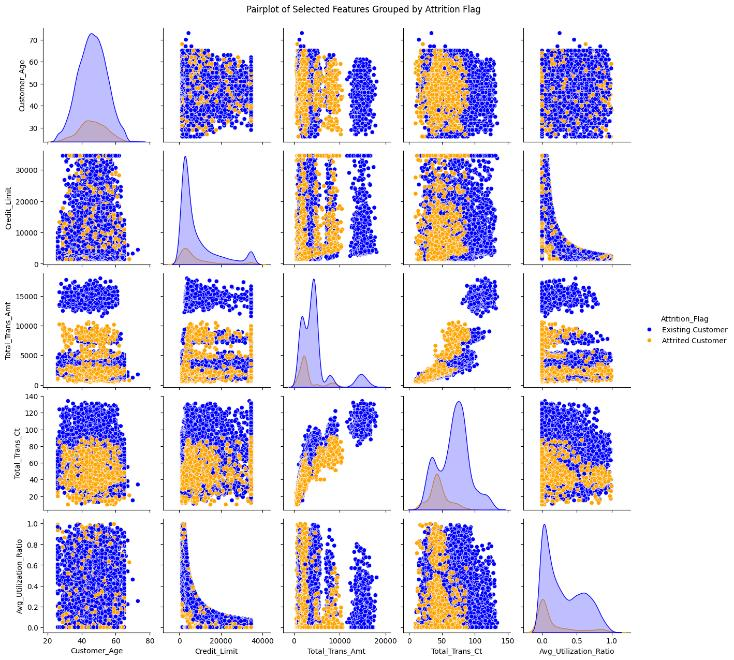
\includegraphics[width=0.4\textwidth]{img/4.png}
\end{figure}

\section{پرسش دوم}

\subsection{پرسش دوم - بخش اول}
داده‌ها را به دو گروه آموزش و آزمون تقسیم می‌کنیم. این کار به منظور ارزیابی بهتر مدل‌ها و پیش‌بینی‌های آن‌ها بر اساس داده‌های جدید انجام می‌شود. در این قسمت، ابتدا داده‌ها را به صورت تصادفی تقسیم کرده و سپس از 70\% آن‌ها برای آموزش مدل و 30\% باقی‌مانده برای ارزیابی عملکرد استفاده خواهیم کرد.

\begin{figure}[!h]
    \centering
    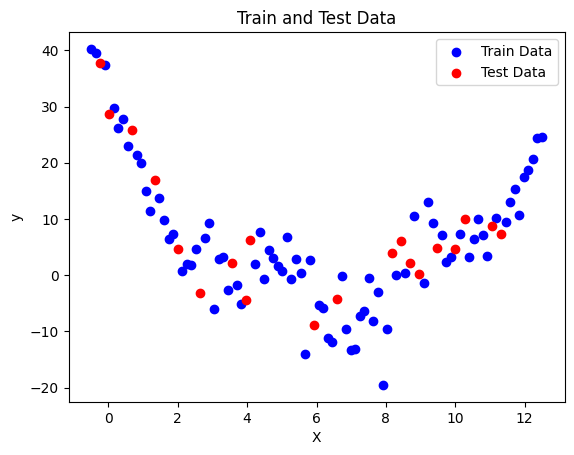
\includegraphics[width=0.4\textwidth]{img/5.png}
\end{figure}

\subsection{پرسش دوم - بخش دوم}
سه معیار رایج برای سنجش عملکرد مدل‌های رگرسیون عبارتند از:

\textbf{خطای میانگین مطلق (MAE)}: این معیار نشان می‌دهد که به طور متوسط، پیش‌بینی مدل چقدر از مقدار واقعی انحراف دارد.
\[
\text{MAE} = \frac{1}{n} \sum_{i=1}^{n} \left| y_i - \hat{y}_i \right|
\]

\textbf{خطای میانگین مربعات (MSE)}: این معیار به میزان تفاوت مربعی بین مقادیر پیش‌بینی شده و واقعی می‌پردازد.
\[
\text{MSE} = \frac{1}{n} \sum_{i=1}^{n} (y_i - \hat{y}_i)^2
\]

\textbf{ضریب تعیین ($R^2$)}: این معیار نشان می‌دهد که مدل چه مقدار از واریانس داده‌ها را توضیح می‌دهد.
\[
R^2 = 1 - \frac{\sum_{i=1}^{n} (y_i - \hat{y}_i)^2}{\sum_{i=1}^{n} (y_i - \bar{y})^2}
\]

\subsection{پرسش دوم - بخش سوم}
در صورتی که داده‌ها به طور واضح دارای رابطه غیرخطی باشند، مدل رگرسیون خطی (درجه اول) قادر به ارائه تخمین دقیقی نخواهد بود. زیرا مدل‌های خطی تنها قادر به مدل‌سازی روابط خطی هستند و نمی‌توانند الگوهای پیچیده‌تر مانند روابط درجه دو را بازسازی کنند. به همین دلیل، استفاده از مدل‌های خطی برای داده‌هایی با روابط غیرخطی ممکن است منجر به خطای زیاد شود.

\subsection{پرسش دوم - بخش چهارم}
در ابتدا، خطای مدل در حالت کلی با افزایش تعداد داده‌های آموزشی کاهش می‌یابد، زیرا مدل می‌تواند بهتر داده‌های آموزش را پیش‌بینی کرده و تطبیق بهتری با آن‌ها پیدا کند. اما پس از رسیدن به یک حد معین از داده‌های آموزشی، خطای آزمون ممکن است افزایش یابد، چرا که مدل ممکن است دچار بیش برازش (Overfitting) شده و نتواند به درستی بر روی داده‌های جدید عمل کند.

\begin{figure}[!h]
    \centering
    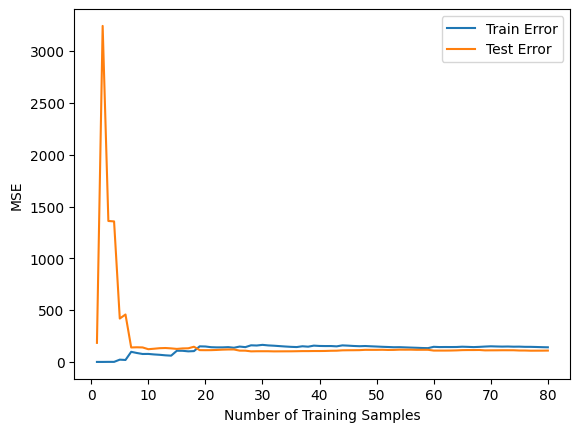
\includegraphics[width=0.4\textwidth]{img/6.png}
\end{figure}

\subsection{پرسش دوم - بخش پنجم}
اگر مدل فعلی دارای خطای بالایی باشد، افزودن داده‌های بیشتر ممکن است به کاهش خطای مدل کمک کند، اما نمی‌توان گفت که خطای مدل به اندازه خطای انسان کاهش خواهد یافت. در صورتی که مدل به دلیل بیش برازش دارای خطای بالا باشد، استفاده از داده‌های بیشتر ممکن است به کاهش خطای مدل کمک کند. اما اگر مدل هنوز نتواند به خوبی الگوهای داده‌ها را یاد بگیرد، ممکن است خطای آن همچنان ثابت بماند.

\begin{figure}[!h]
    \centering
    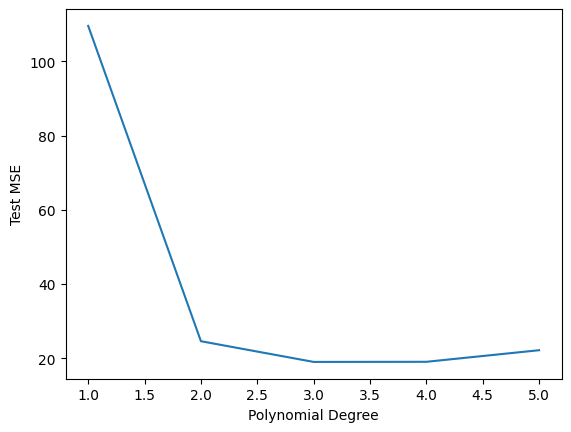
\includegraphics[width=0.4\textwidth]{img/7.png}
\end{figure}

\subsection{پرسش دوم - بخش ششم}
پس از اضافه کردن ویژگی‌های غیرخطی مانند جمله درجه دوم به مدل، خطا به طور چشمگیری کاهش می‌یابد. در این حالت، مدل قادر است رابطه پیچیده‌تر میان ورودی و خروجی را مدل‌سازی کند. با این حال، پس از افزودن ویژگی‌های بیشتر (بالا‌تر از درجه دوم)، تغییرات قابل توجهی در خطای مدل مشاهده نمی‌شود. این نشان‌دهنده اشباع مدل است و بعد از یک حد معین، افزودن ویژگی‌های اضافی تاثیر زیادی بر بهبود مدل نخواهد داشت.

\subsection{پرسش دوم - بخش امتیازی}
برای مقابله با بیش برازش و بهبود توانایی تعمیم مدل، از تکنیک‌های \textit{Regularization} استفاده می‌شود. هدف از regularization، محدود کردن پیچیدگی مدل و جلوگیری از بیش برازش است. در اینجا از دو نوع regularization استفاده خواهیم کرد:

\textbf{Ridge Regression}: این روش یک جریمه به مربعات مقادیر پارامترهای مدل اضافه می‌کند تا از پیچیدگی زیاد مدل جلوگیری شود.
\textbf{Lasso Regression}: این روش جریمه‌ای به مقادیر مطلق پارامترهای مدل اضافه می‌کند و به کاهش ویژگی‌های بی‌اهمیت کمک می‌کند.

\begin{figure}[!h]
    \centering
    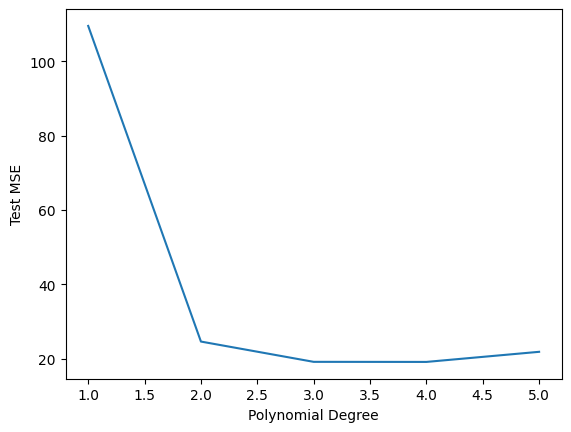
\includegraphics[width=0.4\textwidth]{img/8.png}
\end{figure}

\end{document}
